%%%%%%%%%%%%%%%%%%%%%%%%%%%%%%%%%%%%%%%%%
%
% (c) 2020 by Jennifer Laaser
%
% This work is licensed under the Creative Commons Attribution-NonCommercial-ShareAlike 4.0 International License. To view a copy of this license, visit http://creativecommons.org/licenses/by-nc-sa/4.0/ or send a letter to Creative Commons, PO Box 1866, Mountain View, CA 94042, USA.
%
% The current source for these materials is accessible on Github: https://github.com/jlaaser/pogil-polymers
%
%%%%%%%%%%%%%%%%%%%%%%%%%%%%%%%%%%%%%%%%%

\documentclass[instructor,handout]{pogil}
%\documentclass[handout]{pogil}

%%%%%%%%%%%%%%%%% DOCUMENT INFORMATION %%%%%%%%%%%%%%%%%%%%%%%%

\copyrightshort{\includegraphics[width=0.1\textwidth]{by-nc-sa} J. Laaser 2020}

%%%%%%%%%%%%%%%%%%%%%%%%%%%%%%%%%%%%%%%%%%%%%%%%%%%%%%%%%%%%%%%%%
%%%%%%%%%%%%%%%%%%%%%%%%%%%%%%%%%%%%%%%%%%%%%%%%%%%%%%%%%%%%%%%%%

\begin{document}
	
% to change the activity output in the pdf, change this to the file path for the activity you want to include:
%%%%%%%%%%%%%%%%%%%%%%%%%%%%%%%%%%%%%%%%%%
%
% (c) 2018 by Jennifer Laaser
%
% This work is licensed under the Creative Commons Attribution-NonCommercial-ShareAlike 4.0 International License. To view a copy of this license, visit http://creativecommons.org/licenses/by-nc-sa/4.0/ or send a letter to Creative Commons, PO Box 1866, Mountain View, CA 94042, USA.
%
% The current source for these materials is accessible on Github: https://github.com/jlaaser/pogil-polymers
%
%%%%%%%%%%%%%%%%%%%%%%%%%%%%%%%%%%%%%%%%%

\section{Activity Template}
\renewcommand{\figpath}{content/figs}

\textbf{Focus question:} Put a central question for the students to consider through this exercise here.

\subsection{Model 1:  ABC}

Here is the first model for students to consider

% to include images, put them in the folder specified by figpath and then use:
%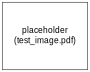
\includegraphics[width=0.8\textwidth]{\figpath/test_image.pdf}

\subsection{Critical Thinking Questions}

	\begin{enumerate}
		\item First question?
		\item Second question?
	\end{enumerate}

\subsection{Model 2: DEF}

\subsection{Critical Thinking Questions}

	\begin{enumerate}
		\item First question?
		\item Second question?
	\end{enumerate}

\subsection{Exercises}

	After class, \textbf{read} the following sections of your textbook:
	
	\begin{enumerate}
		\item First section
		\item Second section
	\end{enumerate}
	
	Then, do the following exercises:
	
	\begin{enumerate}
		\item First exercise
		\item Second exercise
	\end{enumerate}
%%%%%%%%%%%%%%%%%%%%%%%%%%%%%%%%%%%%%%%%%
%
% (c) 2022 by Jennifer Laaser
%
% This work is licensed under the Creative Commons Attribution-NonCommercial-ShareAlike 4.0 International License. To view a copy of this license, visit http://creativecommons.org/licenses/by-nc-sa/4.0/ or send a letter to Creative Commons, PO Box 1866, Mountain View, CA 94042, USA.
%
% The current source for these materials is accessible on Github: https://github.com/jlaaser/pogil-polymers
%
%%%%%%%%%%%%%%%%%%%%%%%%%%%%%%%%%%%%%%%%%

\renewcommand{\figpath}{content}
\renewcommand{\labelbase}{FRPkinetics}

\begin{activity}{Kinetics of Free-Radical Polymerization}
\label{\labelbase}

\begin{instructornotes}
	This activity introduces students to concepts related to the kinetics of free-radical polymerization.
	
	After completing this activity, students will be able to:
	\begin{enumerate}
		\item Write kinetic equations for each of the major steps of a free-radical polymerization
		\item Calculate the kinetic chain length for a free-radical polymerization
		\item Quantify how chain transfer changes the kinetic chain length in a free-radical polymerization
	\end{enumerate}
	
	\subsection*{Activity summary:}
	\begin{itemize}
		\item \textbf{Activity type:} Learning Cycle
		\item \textbf{Content goals:} See above
		\item \textbf{Process goals:} %https://pogil.org/uploads/attachments/cj54b5yts006cklx4hh758htf-process-skills-official-pogil-list-2015-original.pdf
			\begin{itemize}	
				\item Interpreting mathematical relationships
				\item Written and oral communication of reasoning
			\end{itemize}
		\item \textbf{Duration:} 60 minutes, including time for discussion
		\item \textbf{Instructor preparation required:} none beyond knowledge of relevant content
		\item \textbf{Related textbook chapters:}
			\begin{itemize}
				\item \emph{Polymer Chemistry} (Hiemenz \& Lodge), 2nd ed.: sections 3.3.3, 3.4, 3.5.1, 3.8
				\item \emph{Introduction to Polymers} (Young \& Lovell), 3rd ed.: section 4.3
			\end{itemize}
		%\item \textbf{Facilitation notes:}
		%	\begin{itemize}
		%		\item \dots
		%	\end{itemize}
	\end{itemize}
	
\end{instructornotes}


\begin{model}[Kinetic Equations]
	\label{\labelbase:mdl:kineticeqns}

	Rate laws for some common types of chemical reactions are shown below:
	
	\vspace{-6pt}
	\begin{center}
		\renewcommand{\arraystretch}{2}
		\begin{tabular}{c c c c}
			\hspace{2cm}\textbf{Reaction:}\hspace{2cm} & \multicolumn{3}{c}{\hspace{0.5cm}\textbf{Rate laws:}\hspace{0.5cm}} \\
			$ \text{A} \xlongrightarrow{k} \text{B}$ & $\frac{d[\text{A}]}{dt} = -k[\text{A}]$ && $\frac{d[\text{B}]}{dt} = k[\text{A}]$ \\
			$ \text{A} \xlongrightarrow{k} 2\text{ B}$ & $\frac{d[\text{A}]}{dt} = -k[\text{A}]$ && $\frac{d[\text{B}]}{dt} = 2k[\text{A}]$ \\
			$\text{A + B} \xlongrightarrow{k} \text{C}$ & $\frac{d[\text{A}]}{dt} = -k[\text{A}][\text{B}]$ && $\frac{d[\text{C}]}{dt} = k[\text{A}][\text{B}]$ \\
			$\text{2 A} \xlongrightarrow{k} \text{B}$ & $\frac{d[\text{A}]}{dt} = -2k[\text{A}]^2$ && $\frac{d[\text{B}]}{dt} = k[\text{A}]^2$ \\
			$\text{2 A} \xlongrightarrow{k} \text{2 B}$ & $\frac{d[\text{A}]}{dt} = -2k[\text{A}]^2$ && $\frac{d[\text{B}]}{dt} = 2 k[\text{A}]^2$ 
		\end{tabular}
	\end{center}
	Use these rate laws to answer the following questions about the kinetics of free-radical polymerization.
	
\end{model}


\begin{ctqs}

	\question The first step in a free-radical polymerization is initiation.  
		
		\begin{enumerate}
		
			\item First, an initiator molecule decomposes to create initiator radicals: \label{\labelbase:ctq:initdecomp}
				\begin{equation*}
					\text{Init} \xlongrightarrow{k_d} \text{2 \ce{I^.}}
				\end{equation*}	
				Write an expression for the rate at which new initiator radicals are generated, $\frac{d[\text{I}^{\bullet}]}{dt}$, in terms of the concentration of initiator, [Init], and dissociation constant, $k_d$.
		
				\begin{solution}[1in]\instructordisplay{
					\begin{equation*}					
						\frac{d[\text{I}^\bullet]}{dt} = 2k_d[\text{Init}]
					\end{equation*}
				}\end{solution}
		
			\item If a fraction $f$ of the initiator radicals successfully go on to generate new polymer chain radicals (\ce{P^.}), how will the overall initiation rate of polymer chains, $\frac{d[\text{\ce{P^.}}]}{dt}$, be related to the rate of radical generation, $\frac{d[\text{I}^\bullet]}{dt}$?  Use your answer to write an expression for $\frac{d[\text{\ce{P^.}}]}{dt}$ in terms of $f$, $k_d$, and $[\text{Init}]$.
		
				\begin{solution}[1.25in]\instructordisplay{
					\begin{equation*}		
					\frac{d[\text{\ce{P^.}}]}{dt} = f\frac{d[\text{I}^\bullet]}{dt} = 2fk_d[\text{Init}]
					\end{equation*}
					
					Note: the initiator efficiency, $f$, is typically in the range of 0.3 to 0.8.
				}\end{solution}
		
		\end{enumerate}
		
	\question The second step in a free-radical polymerization is propagation:
		\begin{equation*}
			\text{\ce{P_i^.} + M} \xlongrightarrow{k_p} \text{\ce{P_{i+1}^.}}
		\end{equation*}
		
		Generally, we make the approximation that all of the polymer radicals are equally reactive and are ``equivalent'' to each other regardless of chain length, so we summarize this reaction as
		\begin{equation*}
			\text{\ce{P^.} + M} \xlongrightarrow{k_p} \text{\ce{P^.}}
		\end{equation*}
		where [\ce{P^.}] is the \emph{total} concentration of propagating radical chains.
	
		Write an expression for $-\frac{d[\text{M}]}{dt}$, the rate at which monomers are used up, in terms of the radical concentration, [\ce{P^.}], the monomer concentration, [M], and the propagation rate constant, $k_p$.
		
		\begin{solution}[1.25in]\instructordisplay{
			\begin{equation*}
				-\frac{d[\text{M}]}{dt} = k_p [\text{\ce{P^.}}][\text{M}]
			\end{equation*}
		}\end{solution}
		
	\question The final step in a free-radical polymerization is termination:
		\begin{align*}
			\text{\ce{P^.} + \ce{P^.}} \xlongrightarrow{k_{t,c}} \text{\ce{PP}} && \text{or} && \text{\ce{P^.} + \ce{P^.}} \xlongrightarrow{k_{t,d}} \text{P + P}\\
			\text{combination\hspace{0.5cm}} && && \text{disproportionation}
		\end{align*}
		
		\begin{enumerate}
			\item For termination by combination, write an expression for $-\frac{d[\text{P}^{\bullet}]}{dt}$ in terms of the radical concentration, [\ce{P^.}], and the rate constant, $k_{t,c}$.
			
				\begin{solution}[0.75in]\instructordisplay{
					\begin{equation*}
						\left(-\frac{d[\text{\ce{P^.}}]}{dt}\right)_c = 2k_{t,c}[\text{\ce{P^.}}]^2
					\end{equation*}
				}\end{solution}
			
			\item For termination by disproportionation, write an expression for $-\frac{d[\text{P}^{\bullet}]}{dt}$ in terms of the radical concentration, [\ce{P^.}], and the rate constant, $k_{t,d}$.
			
				\begin{solution}[0.75in]\instructordisplay{
					\begin{equation*}
						\left(-\frac{d[\text{\ce{P^.}}]}{dt}\right)_d = 2k_{t,d}[\text{\ce{P^.}}]^2
					\end{equation*}
				}\end{solution}
			
			\item Sum your answers to the previous two questions to find an expression for the \emph{total} rate at which propagating radicals are removed from the reaction, in terms of the total radical concentration, [\ce{P^.}], and the total termination rate constant, $k_t = k_{t,c} + k_{t,d}$.
			
				\begin{solution}[0.75in]\instructordisplay{
					\begin{align*}
						-\frac{d[\text{\ce{P^.}}]}{dt} &= \left(-\frac{d[\text{\ce{P^.}}]}{dt}\right)_c + \left(-\frac{d[\text{\ce{P^.}}]}{dt}\right)_d\\
						&= 2k_{t,c}[\text{\ce{P^.}}]^2 + 2k_{t,d}[\text{\ce{P^.}}]^2\\
						&= 2(k_{t,c} + k_{t,d})[\text{\ce{P^.}}]^2\\
						&= 2k_t[\text{\ce{P^.}}]^2
					\end{align*}
				}\end{solution}
				
		\end{enumerate}

\end{ctqs}



\begin{model}[Summary of Free-Radical Kinetics]
\label{\labelbase:mdl:kineticssummary}

	The major reaction steps in free-radical polymerization and their rate laws are summarized below:
	
	\begin{center}
		\renewcommand{\arraystretch}{2}
		\begin{tabular}{c c c}
			\textbf{Step:} & \textbf{Overall Reaction:} & \textbf{Rate:}\\\hline
			\multirow{2}{*}{Initiation} & $[\text{Init}] \xlongrightarrow{k_d} \text{2 \ce{I^.}}$ & \multirow{2}{*}{$ R_i = \frac{d\text{[\ce{P^.}]}}{dt} = 2fk_d[\text{Init}]$}\\
			 & $\text{\ce{I^.} + M} \xlongrightarrow{k_i} \text{\ce{P^.}}$ & \\\hline
			Propagation & $\text{\ce{P^.} + M} \xlongrightarrow{k_p} \text{\ce{P^.}}$ & $R_p = -\frac{d[\text{M}]}{dt} = k_p\text{[M][\ce{P^.}]}$\\\hline
			\multirow{2}{*}{Termination} & $\text{\ce{P^.} + \ce{P^.}} \xlongrightarrow{k_{t,c}} \text{\ce{PP}}$ & \multirow{2}{*}{$R_t = -\frac{d[\text{\ce{P^.}}]}{dt} = 2k_t [\text{\ce{P^.}}]^2$}\\
			& $\text{\ce{P^.} + \ce{P^.}} \xlongrightarrow{k_{t,d}} \text{P + P}$ & \\\hline
		\end{tabular}
	\end{center}
	\vspace{6pt}

\end{model}

\begin{ctqs}

	\question Which rate ($R_i$, $R_p$, or $R_t$) describes...
	
		\begin{enumerate}
			\item ... the rate at which new propagating polymer radicals are generated?
			
				\begin{solution}[0.4in]
					$R_i$
				\end{solution}
				
			\item ... the rate at which monomers are incorporated into polymer?
			
				\begin{solution}[0.4in]
					$R_p$
				\end{solution}
				
			\item ... the rate at which propagating polymer radicals are removed from the reaction?
			
				\begin{solution}[0.4in]
					$R_t$
				\end{solution}
				
		\end{enumerate}

	\question To simplify the kinetic equations shown in Model \ref{\labelbase:mdl:kineticssummary}, we assume that the concentration of radicals reaches a ``steady state'', where [\ce{P^.}] is constant.
	
		\begin{enumerate}
			\item One way to ensure that $[\text{P}^{\bullet}]$ reaches a steady state is to require that the rate at which polymer radicals are \emph{generated} is equal to the rate at which they are \emph{removed} from the reaction.
			
				Which two rates ($R_i$, $R_p$, and/or $R_t$) must be equal for this to be true?
				
				\begin{solution}[0.75in]
					$R_i$ and $R_t$ (i.e. we need $R_i=R_t$)
				\end{solution}
				
			\item Set the two rates identified in the previous question equal to each other and solve for the steady state radical concentration $[\text{P}^{\bullet}]$ in terms of $f$, $k_d$, $k_t$, and $[\text{Init}]$.
			
				\begin{solution}[2in]
					\begin{align*}
						R_i &= R_t \\
						2fk_d[Init] &= 2k_t[P^\bullet]^2\\
						[P^\bullet]^2 &= \frac{fk_d[Init]}{k_t}\\
						[P^\bullet] &= \left(\frac{fk_d[Init]}{k_t}\right)^{1/2}
					\end{align*}
				\end{solution}
			
			\item Finally, use your answer to find an expression for the polymerization rate, $R_p$, in terms of $f$, $k_d$, $k_p$, $k_t$, $[\text{M}]$, and $[\text{Init}]$. \label{\labelbase:ctq:Rp}
			
				\begin{solution}[1.5in]\instructordisplay{
					\begin{align*}
						R_p &= k_p\text{[M][\ce{P^.}]}\\
						&= k_p\text{[M]}\left(\frac{fk_d[Init]}{k_t}\right)^{1/2}
					\end{align*}
					\emph{Note: the integrated form of this rate law is given in Exercise \ref{\labelbase:exc:integratedrate}.}
				}\studentdisplay{~}\end{solution}
			
		\end{enumerate}
	
	\question Consider a period of time, $\Delta t$, after the reaction has reached its steady state.
	
		\begin{enumerate}
			
			\item How many monomers do you expect to be incorporated into polymer chains in this time interval?  Give your answer in terms of $R_i$, $R_p$, $R_t$, and/or $\Delta t$.
			
				\begin{solution}[0.5in]
				
					$R_p \Delta t$
					
				\end{solution}
			
			\item How many new polymer chains do you expect to be generated in this time interval?  Give your answer in terms of $R_i$, $R_p$, $R_t$, and/or $\Delta t$.
			
				\begin{solution}[0.5in]
				
					$R_i \Delta t$
					
				\end{solution}
			
			\item Based on your answers to the preceding two questions, what should the average length of the polymer chains generated in this interval be?
			
				\begin{solution}[0.75in]
				
					Average length = $\frac{\text{number of monomers}}{\text{number of chains}} = \frac{R_p\Delta t}{R_i \Delta t} = \frac{R_p}{R_i}$				
				
				\end{solution}
				
		\end{enumerate}
	
\end{ctqs}

\begin{infobox}\label{\labelbase:infobox:kineticchainlength}
	The \emph{kinetic chain length}, $\bar v$, is the ratio of the propagation rate to the initiation (or termination) rate:
	\begin{equation*}
		\bar v = \frac{R_p}{R_i} = \frac{R_p}{R_t}
	\end{equation*}
	This value equals the average number of monomers that add to each propagating radical before it terminates.
\end{infobox}

\begin{ctqs}

	\question Substitute in appropriate expressions for $R_p$ and $R_i$ to find an expression for $\bar v$ in terms of the rate constants $k_d$, $k_p$, and $k_t$, and the concentrations of monomer and initiator.
	
		\begin{solution}[2.5in]\instructordisplay{
			\begin{align*}
				\bar v &= \frac{R_p}{R_i} = \frac{k_p [M] \sqrt{f\frac{k_d}{k_t}[\text{Init}]}}{2fk_d[\text{Init}]}\\
					&= \frac{k_p[\text{M}]}{2}\sqrt{\frac{1}{f k_d k_t [\text{Init}]}}
			\end{align*}
		}\end{solution}
		
	\question Based on what you know about the relevant reactions, propose equations relating the final number-average degree of polymerization ($N_n$) of the terminated polymer chains to the kinetic chain length ($\bar v$) of the propagating radicals for...
		
		\begin{enumerate}
		
			\item ... polymers that terminate by disproportionation:
			
				\emph{Hint: does termination by disproportionation change the lengths of the chains?  If so, how?}
				
				\begin{solution}[0.75in]
					Termination by disproportionation does not change the length of the chains, so we should have 
					
					$N_n = \bar v$
				\end{solution}
			
			\item ... polymers that terminate by combination:
			
				\emph{Hint: does termination by combination change the lengths of the chains?  If so, how?}
				
				\begin{solution}[0.75in]
					Termination by combination effectively doubles the length of the chains, so we should have 
					
					$N_n = 2\bar v$
				\end{solution}
		
		\end{enumerate}

\end{ctqs}

		
\clearpage
\begin{model}[Chain Transfer]
\label{\labelbase:mdl:chainxfer}

	In Models \ref{\labelbase:mdl:kineticeqns} and \ref{\labelbase:mdl:kineticssummary}, we considered the intiation, propagation, and termination steps of a free-radical polymerization.  However, in practice, chain transfer often matters too.
	
	For a chain transfer reaction that transfers the propagating radical to some other species, RX,
	\begin{align*}
		\text{\ce{P^.} + RX} \xlongrightarrow{k_{tr}} \text{PX + \ce{R^.}}
	\end{align*}
	the chain-transfer rate obeys
	\begin{align*}
		R_{tr} = -\frac{d[\text{\ce{P^.}}]}{dt} = k_{tr}\text{[\ce{P^.}][RX]}
	\end{align*}
	
\end{model}

\begin{ctqs}
	\question As shown in Model \ref{\labelbase:mdl:chainxfer}, chain-transfer \emph{effectively} terminates a polymer radical \ce{P^.}.  This process occurs \emph{in addition} to the bimolecular termination processes discussed in the previous model.
	
		\begin{enumerate}
			\item Propose an expression for the total \emph{effective} termination rate, $R_{t,eff}$, that takes both of these processes into account.
		
		\begin{solution}[0.5in]
	
			\begin{equation*}
				R_{t,eff} = R_t + R_{tr}
			\end{equation*}
	
		\end{solution}
			
			\item Replace $R_t$ in the equation for $\bar v$ given in the information box on page \pageref{\labelbase:infobox:kineticchainlength} with your answer to the previous question to obtain an expression for the kinetic chain length in the presence of chain transfer, $\bar v_{tr}$, in terms of $R_p$, $R_t$, and $R_{tr}$.
		
		\begin{solution}[0.5in]
	
			\begin{equation*}
				\bar v_{tr} = \frac{R_p}{R_{t,eff}}  = \frac{R_p}{R_t + R_{tr}}
			\end{equation*}
	
		\end{solution}
		
		\end{enumerate}
		
\end{ctqs}

\begin{infobox}
\label{\labelbase:info:vtr}

	It is possible to show (see Exercise \ref{\labelbase:exc:chainxfer}) that for a system that contains multiple species RX that can participate in chain-transfer reactions, the kinetic chain length in the presence of chain-transfer ($\bar v_{tr}$) is related to the kinetic chain length in the absence of chain transfer ($\bar v$) by
	\begin{align*}
		\frac{1}{\bar v_{tr}} = \frac{1}{\bar v} + \sum_{\text{all RX}} C_{RX}\frac{\text{[RX]}}{\text{[M]}}
	\end{align*}
	where
	\begin{align*}
		C_{RX} = \frac{k_{tr,R}}{k_p}
	\end{align*}
	is the ``chain transfer constant'' for the species RX.
	
\end{infobox}

\begin{ctqs}

	\question Does this equation tell you that chain transfer will generally \emph{increase} or \emph{decrease} the length of the polymer chains?  Justify your group's answer in 1-2 complete sentences.
	
		\begin{solution}[2in]
			This equation tells us that chain transfer should decrease the length of the polymer chains relative to the chain length that would be obtained in the absence of chain transfer.  The equation tells us that $1/\bar v_{tr}$ is larger than $1/\bar v$ (at least, as long as $C_{RX}$ is positive!), so $\bar v_{tr}$ will be smaller than $\bar v$.
		\end{solution}
		
	\question If there is only a \emph{single} species RX that participates in chain-transfer, the equation for $v_{tr}$ simplifies to
	\begin{align*}
		\frac{1}{\bar v_{tr}} = \frac{1}{\bar v} + C_{RX}\frac{\text{[RX]}}{\text{[M]}}
	\end{align*}
		Propose an experiment that you could do to measure the chain-transfer constant, $C_{RX}$.
		
		\begin{solution}[2.5in]
			To measure the chain-transfer constant, $C_{RX}$, we could perform polymerizations with different amounts of the species RX.  Fitting $1/\bar v_{tr}$ vs. $[RX][M]$ would give a straight line whose slope is the the chain transfer constatn $C_{RX}$.
		\end{solution}
	
\end{ctqs}


\begin{exercises}
		
	\exercise In this activity, two major assumptions were made about the polymerization kinetics: first, that all propagating radicals are equivalent, regardless of chain length; and second, that the reaction reaches a steady-state radical concentration.
	
		Are these assumptions reasonable?  Justify your answer.
			
				\begin{solution}\instructordisplay{
					These assumptions are probably reasonable.  Regarding the equivalence of the propagating radicals, there may be some dependence of the propagation rates on the chain lengths, but the biggest differences occur when the chains are very short. Since free radical polymerizations typically reach very long chain lengths, most of the polymerization will be in the regime where it is reasonable to assume equal reactivity.
					
					Regarding the assumption of steady-state concentration, it typically only takes a few seconds for the reaction to approach its steady state radical concentration.  After this point, the kinetics are self-correcting: if there is too much initiation, $[P^\bullet]$ increases and so $R_t$ (which goes as $[P^\bullet]^2$ increases) to bring the concentration of active chains back down.  Conversely, if there is too little initiation, $R_t$ decreases until the concentration of active chains comes back up.  So, as long as the reaction time is long enough relative to the initial period in which the kinetics ramp up, most of the reaction will proceed in the steady state limit.  
				}\end{solution}
		
	\exercise Derive the expression for $\frac{1}{\bar v_{tr}}$ given on page \pageref{\labelbase:info:vtr} by doing the following:
	
		\label{\labelbase:exc:chainxfer}
		
		\begin{enumerate}
			\item Write an expression for the total chain-transfer rate, $R_{tr}$, as a sum over all species RX.
			
				\begin{solution}\instructordisplay{
					\begin{equation*}
						R_{tr} = \sum_{RX} k_{tr,RX}[\text{\ce{P^.}}][\text{RX}]
					\end{equation*}
				}\end{solution}
				
			\item Substitute this expression, and appropriate expressions for $R_p$ and $R_t$, into $\bar v_{tr} = \frac{R_p}{R_t + R_{tr}}$.  Then calculate $\frac{1}{v_{tr}}$.
			
				\begin{solution}\instructordisplay{
					\begin{align*}
						\bar v_{tr} = \frac{R_p}{R_t + R_{tr}}
							&= \frac{R_p}{R_t + \sum_{RX} k_{tr,RX}[\text{\ce{P^.}}][\text{RX}]}\\
						\frac{1}{\bar v_{tr}} &= \frac{R_t + \sum_{RX} k_{tr,RX}[\text{\ce{P^.}}][\text{RX}]}{R_p}
					\end{align*}
				}\end{solution}
				
			\item Finally, simplify your equation for $\frac{1}{v_{tr}}$ to obtain the expression on page \pageref{\labelbase:info:vtr}.
			
				\emph{Hint: you will need the expression for $R_p$ from Model \ref{\labelbase:mdl:kineticssummary}.}
			
				\begin{solution}\instructordisplay{
					\begin{align*}
						\frac{1}{v_{tr}} &= \frac{R_t + \sum_{RX} k_{tr,RX}[\text{\ce{P^.}}][\text{RX}]}{R_p}\\
							&= \frac{R_t}{R_p} + \frac{\sum_{RX} k_{tr,RX}[\text{\ce{P^.}}][\text{RX}]}{R_p}\\
							&= \frac{1}{\bar v} + \sum_{RX} \frac{k_{tr,RX}}{R_p}[\text{\ce{P^.}}][\text{RX}]
					\end{align*}
				}\end{solution}	% necessary to avoid an awkward page break
				\begin{solution}\instructordisplay{
				Recalling that $R_p = k_p [M][\text{\ce{P^.}}]$,
					\begin{align*}
						\frac{1}{v_{tr}} &= \frac{1}{\bar v} + \sum_{RX} \frac{k_{tr,RX}}{k_p [M][\text{\ce{P^.}}]}[\text{\ce{P^.}}][\text{RX}]\\
							&= \frac{1}{\bar v} + \sum_{RX} \frac{k_{tr,RX}}{k_p} \frac{[\text{RX}]}{[\text{M}]}\\
							&= \frac{1}{\bar v} + \sum_{RX} C_{RX} \frac{[\text{RX}]}{[\text{M}]}
					\end{align*}
					as desired.
				}\end{solution}
				
		\end{enumerate}
		
	\exercise In this activity, you explored the differential forms of the rate laws for free radical polymerization.   However, it is also useful to obtain explicit expressions for the amount of polymer generated as a function of time.
	
		\begin{enumerate}
			\item In CTQ \ref{\labelbase:ctq:initdecomp}, you obtained an expression for $\frac{d[I^\bullet]}{dt}$.  Write an analogous expression for $\frac{d[\text{Init}]}{dt}$.  Then, assuming the initial initiator concentration is $[\text{Init}]_0$, derive an expression for $[\text{Init}]$ as a function of time.
			
				\begin{solution}\instructordisplay{
					Referencing the table in Model \ref{\labelbase:mdl:kineticeqns}, we can write
					\begin{equation*}
						-\frac{d[\text{Init}]}{dt} = k_d[\text{Init}]
					\end{equation*}
					Rearranging and integrating, we find
					\begin{align*}
						\frac{1}{[\text{Init}]}\frac{d[\text{Init}]}{dt} &= -k_d\\
							\frac{d(\ln [\text{Init}])}{dt} &= -k_d\\
							\ln[\text{Init}] &= \int -k_d \, dt + C\\
							\ln[\text{Init}] &= -k_d t + C\\
							[\text{Init}] &= e^{-k_d t + C}\\
								&= A e^{-k_d t}
					\end{align*}
					Since we are told that the initial initiator concentration is $[\text{Init}]_0$, we can solve for the integration constant $A$ using
					\begin{align*}
						[\text{Init}]_0 &= A e^{-k_d \cdot 0}\\
						[\text{Init}]_0 &= A
					\end{align*}
					Thus, 
					\begin{equation*}
						[\text{Init}] = [\text{Init}]_0 e^{-k_d t}
					\end{equation*}
				}\end{solution}
			
			\item \label{\labelbase:exc:integratedrate} Combine this result with the expression for $R_p$ derived in CTQ \ref{\labelbase:ctq:Rp} and integrate the result to show that the fraction of monomer remaining at time $t$ obeys
				\begin{equation*}
					-\ln\left(\frac{[M]}{[M]_0}\right) = 2k_p\left(\frac{f[Init]_0}{k_d k_t}\right)^{1/2}\left(1-e^{-k_d t/2}\right)
				\end{equation*}
				
				\emph{Hint: you may find it useful to recall that $\frac{1}{x}\frac{dx}{dt} = \frac{d(\ln(x))}{dt}$.}
			
				\begin{solution}\instructordisplay{
					As shown in CTQ \ref{\labelbase:ctq:Rp},
					\begin{align*}
						R_p = -\frac{d[\text{M}]}{dt} = k_p\text{[M]}\left(\frac{fk_d[Init]}{k_t}\right)^{1/2}
					\end{align*}
					Substituting in the above expression for $[\text{Init}]$, we obtain
					\begin{align*}
						-\frac{d[\text{M}]}{dt} = k_p\text{[M]}\left(\frac{fk_d[\text{Init}]_0 e^{-k_d t}}{k_t}\right)^{1/2}
					\end{align*}
					Again, rearranging to put all of the $[M]$'s on one side and all of the $t$'s on the other side, we obtain
					\begin{align*}
						\frac{1}{[M]}\frac{d[M]}{dt} &= -k_p\left(\frac{fk_d[\text{Init}]_0 e^{-k_d t}}{k_t}\right)^{1/2}\\
						\frac{d(\ln [M])}{dt} &= -k_p\left(\frac{fk_d[\text{Init}]_0 }{k_t}\right)^{1/2}e^{-k_d t/2}
					\end{align*}
					Integrating, we obtain
					\begin{align*}
						\ln [M] &= -k_p\left(\frac{fk_d[\text{Init}]_0 }{k_t}\right)^{1/2} \int e^{-k_d t/2} \, dt + C\\
						\ln [M] &= -k_p\left(\frac{fk_d[\text{Init}]_0 }{k_t}\right)^{1/2} \frac{-2}{k_d} e^{-k_d t/2} + C\\
						\ln [M] &= 2k_p\left(\frac{f[\text{Init}]_0 }{k_t k_d}\right)^{1/2} e^{-k_d t/2} + C
					\end{align*}
					Finally, recognizing that the initial condition is that $[M] = [M]_0$ at $t=0$, we can solve for the integration constant $C$:
					\begin{align*}
						\ln [M]_0 &= 2k_p\left(\frac{f[\text{Init}]_0 }{k_t k_d}\right)^{1/2} e^{-k_d 0/2} + C\\
						\ln [M]_0 &= 2k_p\left(\frac{f[\text{Init}]_0 }{k_t k_d}\right)^{1/2} + C\\
						C &= \ln [M]_0 - 2k_p\left(\frac{f[\text{Init}]_0 }{k_t k_d}\right)^{1/2} 
					\end{align*}
					Combining these results, we obtain
					\begin{align*}
						\ln [M] &= 2k_p\left(\frac{f[\text{Init}]_0 }{k_t k_d}\right)^{1/2} e^{-k_d t/2} + \ln [M]_0 - 2k_p\left(\frac{f[\text{Init}]_0 }{k_t k_d}\right)^{1/2}\\
						\ln[M]_0 - \ln[M] &= 2k_p\left(\frac{f[\text{Init}]_0 }{k_t k_d}\right)^{1/2} - 2k_p\left(\frac{f[\text{Init}]_0 }{k_t k_d}\right)^{1/2} e^{-k_d t/2} \\
						-\ln\frac{[M]}{[M]_0} &= 2k_p\left(\frac{f[\text{Init}]_0 }{k_t k_d}\right)^{1/2} \left(1- e^{-k_d t/2} \right)
					\end{align*}
					as desired.
				}\end{solution}
				
			\item Often, the progress of a reaction is reported as a ``percent conversion'', i.e. it is reported in terms of the percentage of monomers that have been converted to polymer.  Derive an expression for the percent conversion of a free-radical polymerization as a function of time in terms of the rate constants $k_p$, $k_d$, $k_t$, the initiator efficiency $f$, and the initial initiator concentration, $[\text{Init}]_0$.
			
				\begin{solution}\instructordisplay{
					The fraction of monomer remaining at time $t$ is
					\begin{align*}
						\text{fraction of monomer remaining} = \frac{[M]}{[M]_0}
					\end{align*}
					The fraction of monomer converted is just 1 minus this fraction
					\begin{align*}
						\text{fraction of monomer converted} &= 1- \frac{[M]}{[M]_0}\\
						&= 1 - e^{- 2k_p\left(\frac{f[\text{Init}]_0 }{k_t k_d}\right)^{1/2} \left(1- e^{-k_d t/2} \right)}
					\end{align*}
					Finally, the percent conversion is just 100\% times this quantity.
				}\end{solution}
		\end{enumerate}
		
%	\exercise A problem on radical lifetimes?	-- Alternatively, could be an Extension activity, or a great exam problem!
		% could essentially start by saying, rate at which monomer is incorp'd into ALL chains is k_p[M][P] if the conc. of propagataing chains is [P], what is the rate at which monomer is incorp'd into a single chain? (k_p [M]).  Then, how long does it take to reach kinetic chain length v?  And assuming chains terminate when they reach v, how long does an individual radical live for?  Finally, have them calculate based on reasonable constants for FRP and compare to step-growth.

	%\exercise a problem on temperature dependence of rates?  -- Alternatively, could be an extension activity

	%\exercise some sort of qualitative question re. Trommsdorff effect?
	
\end{exercises}



%\begin{problems}
%
%	\problem First exercise
%	\problem Second exercise
%	
%\end{problems}


	
\end{activity}


\end{document}
